\documentclass[11pt]{extarticle}
\usepackage{manualdoprofessor}
\usepackage{fichatecnica}
\usepackage{lipsum,media9}
\usepackage[justification=raggedright]{caption}
\usepackage[one]{bncc}
\usepackage[araucaria]{../edlab}
\usepackage{marginnote}
\usepackage{pdfpages}
\usepackage[printwatermark]{xwatermark}
%\newwatermark[pagex=2]{\includegraphics{testc.png}}
%\newwatermark[oddpages]{\includegraphics{test.png}}
%\newwatermark[evenpages]{\includegraphics{testb.png}}

\pagecolor{cyan!0!magenta!10!yellow!28!black!28!}


\newcommand{\AutorLivro}{Camila Werner}
\newcommand{\TituloLivro}{Esconde-esconde}
\newcommand{\Tema}{Jogos; brincadeiras e diversão}
\newcommand{\Genero}{Prescritivos: instruções; guias; manuais; ciclo de crescimento; ciclo de vida etc}
%\newcommand{\imagemCapa}{./images/PNLD0001-01.png}
\newcommand{\issnppub}{978-65-99448-15-7}
\newcommand{\issnepub}{978-65-99448-16-4}
% \newcommand{\fichacatalografica}{PNLD0001-00.png}
\newcommand{\colaborador}{Paulo Pompermaier e Renier Silva}

\begin{document}

\title{\TituloLivro}
\author{\AutorLivro}
\def\authornotes{\colaborador}

\date{}
\maketitle

%\begin{abstract}\addcontentsline{toc}{section}{Carta ao professor}
%\pagebreak

\tableofcontents



\section{Sobre o livro}

%550 caracteres
\paragraph{O livro} \textit{Esconde-esconde}, de Camila Werner, traz diferentes animais, da fauna brasileira e mundial, nas mais diversas cores e texturas. A cada página, o leitor é convidado a interagir com a obra, sendo perguntado onde está determinado animal em cada página. Para isso, a narrativa não se apoia apenas na espécie do animal, mas nas suas cores, que são muito diversificas: não têm uma cor sólida, mas estão cheios de pintinhas, listras e manchas. O livro, assim, configura-se como uma verdadeira brincadeira de esconde-esconde, na qual os animais se misturam e portam cores lúdicas e fantásticas.


%822 caracteres
\paragraph{Descrição} \textit{Esconde-esconde} traz diversas espécies de animais e insetos: girafa, borboleta, joaninha, jacaré, vaca, bezerro, zebra, cobra, onça, pato e tigre. Eles sempre aparecem agrupados durante a narrativa, sendo cada dupla de páginas dedicada a uma espécie. Em cada dupla também aparece uma pergunta para que o leitor observe os animais daquela página e interaja com as ilustrações, tentando encontrar, dentre os animais figurados, aquilo que foi proposto no texto escrito. Entre vários jacarés, por exemplo, o leitor é convidado a encontrar qual é o verde. Ou, entre vacas e bezerros, encontrar a vaca e seu filhote malhados. Através das cores dos animais, uma página também dialoga com a outra.
Por exemplo, há uma página com vários patos coloridos, e pergunta-se do que os patos estão fantasiados: alguns estão com os padrões de cores das joaninhas, outros com as manchas do tigre, um com as listras da zebra. 
A forma como as páginas estão estruturadas também remetem ao zigue-zague do esconde-esconde: a cada dupla de páginas as figuras trocam de lugar. Em uma página, o texto fica ao lado esquerdo e a figura ao lado direito, e na dupla seguinte as posições se invertem, sendo que as ilustrações estão na esquerda e o texto ao lado direito. Isso é interessante pois torna o livro interativo, imprimindo uma dinâmica ao passar de páginas.

%411 caracteres
\paragraph{Competências}
O livro \textit{Esconde-esconde} permite trabalhar e explorar diversas competências com as crianças. Como é dinâmico, já pressupõe um diálogo entre o leitor e a obra, explorando a oralidade e a verbalização de ideias. Quando a criança se envolve no jogo, procurando as respostas, exercita a capacidade de reconhecimento, observação e discriminação, pois deve observar atentamente as figuras para discriminar aquelas com as características enunciadas no texto. Como envolve a imaginação e percepção da criança, essa dinâmica aprofunda sua capacidade de identificar personagens e perceber suas características próprias, uma competência fundamental para o bom aproveitamento de qualquer narrativa.


%862 caracteres
\paragraph{Aprofundamento} Este material tem a 
intenção de contribuir para que você consiga desenvolver um trabalho aprofundado 
com esta obra na sala de aula. Você encontrará informações sobre a autora, sobre 
o gênero e sobre os temas trabalhados ao longo do livro. Apresentaremos também 
algumas propostas de trabalho para a sala de aula que você poderá explorar livremente, 
da forma que considerar mais apropriada para os seus estudantes. Para a prática 
da Literacia Familiar, oferecemos um guia que pode ajudar nas orientações aos 
responsáveis pela criança, para incentivar o gosto pela leitura e contribuir para 
que os estudantes desenvolvam em casa habilidades que serão importantes no momento 
da alfabetização. Por fim, você encontrará sugestões de livros, artigos e sites 
selecionados para enriquecer a sua experiência de leitura e, 
consequentemente, a de seus estudantes.



\section{Sobre os autores}

%532 caracteres
\paragraph{A autora} 

%313 caracteres
\paragraph{Publicações}

%358 caracteres
\paragraph{Currículo} 


\section{Sobre o gênero}

%55 caracteres
\paragraph{O gênero} O gênero deste livro é \textit{prescritivo}. 

%596 caracteres
\paragraph{Descrição} O livro pode ser classificado no gênero prescritivo pois, com a brincadeira do esconde-esconde, ele ensina à criança as diferentes características dos animais: que as joaninhas são vermelhas com pintinhas pretas; que a zebra é listrada; que o tigre é mais laranja, enquanto a onça é mais amarela etc. A principal função desse gênero, portanto, pode ser definida como instruir o leitor.
Extremamente comum na vida quotidiana, é um gênero presente
sempre que se precisa de uma guia ou uma orientação. São estruturas 
que oferecem padrões: leis, que podem ser jurídicas, como um código
penal, ou gramaticais, como um dicionário ou uma gramática; a constituição
de um país etc. Seu conteúdo é, de alguma forma, imutável, ao menos até que seja
mudado. O significado de uma palavra no dicionário deve continuar o mesmo
até que um novo seja adicionado. Enquanto isso, o texto
estabelecido será aquele que tem valor absoluto.

%603 caracteres
\paragraph{Interação} De forma lúdica e descontraída, a obra ajuda a instruir a criança no conhecimento sobre diferentes animais, mostrando seus padrões de cores, as palavras para denominar tais cores e padrões etc. Ademais, é um gênero fundamental para a estruturação da sociedade.
Sempre estamos recorrendo a obras prescritivas, em geral de consulta, para
sabermos como devemos agir: seja uma dúvida a respeito da ortografia ou 
dos significados de uma palavra, seja a respeito de um direito ou dever
enquanto cidadão. É de extrema importância, portanto, que as crianças
sejam o mais cedo apresentadas a este gênero, ainda que com a 
devida abordagem lúdica que a idade demanda.

%862 caracteres
\paragraph{Competências} Em um livro como
\emph{Esconde-esconde}, trabalhamos diversas competências relacionadas ao gênero prescritivo. 
Primeiro, há uma apresentação à necessidade de se fazer as coisas de um 
determinado jeito. É o mundo das regras e convenções sociais: há uma determinada cor a ser encontrada e definida para cada animal. Quando o pato está de vermelho com pintinhas pretas, por exemplo, está se disfarçando de joaninha, pois essa é a cor característica do inseto. As palavras representam animais, que também vêm representados com desenhos, levando-nos a uma segunda competência: a associação entre os traços gráficos e as ilustrações. As cores, nesse livro, são fundamentais para esse processo, pois criam relações de similitude e diferenciação entre os animais (entre o tigre e a onça, por exemplo, a principal diferença é a cor). Ainda que pareça ser um gênero
limitante, são os conhecimentos fixados nestas obras que permitem a expansão
da criatividade com a garantia de que o outro irá entender, já que as convenções são comuns.


\section{Temas}

\subsection{Jogos; brincadeiras e diversão}

%136 caracteres
\paragraph{Abordagem} O livro relaciona-se ao universo lúdico dos jogos. Como indicado já no título, trata-se da brincadeira do esconde-esconde: os animais estão escondidos nas páginas e cabe ao leitor tomar parte no jogo para encontrá-los.

%206 caracteres
\paragraph{Descrição} Através dessa brincadeira, apresenta-se uma ótima oportunidade para trabalhar a percepção, observação, atenção e capacidade de discriminação entre diferentes características. Em cada dupla de páginas, uma nova brincadeira é apresentada no jogo de esconde-esconde, tornando a leitura dinâmica e interativa.

%275 caracteres
\paragraph{Competências} Este tema relaciona-se, principalmente, ao 
campo da experiência Espaços, tempos, quantidades, relações e transformações 
descrito pela \textsc{bncc}, que explora a capacidade da criança de observar as propriedades e características dos objetos ao seu redor e conseguir estabelecer continuidades e rupturas entre eles, apreendendo as dimensões do objeto e classificando-os.

\subsection{Animais da fauna local nacional e mundial}

%136 caracteres
\paragraph{Abordagem} Na brincadeira de esconde-esconde, os protagonistas são os animais. 
Todas as brincadeiras e jogos de encontrar envolvem animais e insetos.

%206 caracteres
\paragraph{Descrição} O livro oferece uma ótima oportunidade de explorar 
as características destes animais com as crianças, além de abrir espaço para uma 
conversa sobre outros animais que façam parte do repertório dos estudantes. 

%275 caracteres
\paragraph{Competências} Este tema relaciona-se, igualmente, ao 
campo da experiência Espaços, tempos, quantidades, relações e transformações 
descrito pela \textsc{bncc}, que explora a curiosidade infantil sobre o mundo 
para proporcionar a construção de conhecimento a partir da observação e exploração. 


\section{Modelagem de aula}
A seguir você encontrará a descrição de uma aula modelo como exemplo 
prático de exploração do livro com estudantes. Esta seção apresentará 
orientações sobre como organizar a sala de aula para receber os 
estudantes, exercitar a interação verbal e prepará-los para o 
momento da leitura.

Em seguida, você encontrará a \textbf{Leitura dialogada}, um 
tópico destinado a te orientar para o momento específico da 
leitura com os estudantes. Por fim, no tópico 
\textbf{Propostas de atividades}, você encontrará ideias 
de práticas que pode explorar com as crianças em sala de 
aula antes, após e durante a leitura. 

Essas atividades podem ser trabalhadas de acordo com a 
disponibilidade do seu cronograma. Fique à vontade para adaptá-las 
da forma que achar melhor para os seus estudantes. Cada turma é única 
e o seu conhecimento prático das características de cada aluno será 
essencial para definir a melhor forma de aplicar essas ideias. 

O objetivo deste manual é oferecer algumas ideias 
e inspirações para um trabalho que pode ser desenvolvido tanto 
a curto, quanto a médio e longo prazo. Sinta-se à vontade para 
personalizar a aula e torná-la sua, aplicando seus conhecimentos, sua 
personalidade e aproveite para fortalecer 
seu vínculo com a turma.


\subsection{Antes de ler}

\BNCC{EI02EF01}
\BNCC{EI02CG02}
\BNCC{EI02ET04}
\BNCC{EI02EO05}
\BNCC{EI02EO06}

%Alterar o nível escolar nesse parágrafo.
Como este trabalho será realizado com crianças da \textbf{Creche 2}, 
que ainda não têm tanta intimidade com o livro enquanto objeto, você terá o 
papel essencial de mediar este contato. 

Nosso objetivo é que os próprios estudantes possam manusear 
e explorar o livro de forma autônoma, mas, para que isto aconteça, você 
pode ajudar a tornar o caminho mais convidativo com atividades que tenham 
intencionalidade educativa. 

A \textsc{bncc} define intencionalidade educativa como ``organização 
e proposição, pelo educador, de experiências que permitam às crianças 
conhecer a si e ao outro e de conhecer e compreender as relações com a 
natureza, com a cultura e com a produção científica, que se traduzem nas 
práticas de cuidados pessoais (alimentar-se, vestir-se, higienizar-se), 
nas brincadeiras, nas experimentações com materiais 
variados, na aproximação com a literatura e no encontro com as 
pessoas''.\footnote{\textsc{bncc}, página 39}

É importante manter essa intencionalidade em mente não apenas na condução 
das atividades propostas neste manual, mas também para aproveitar as 
oportunidades espontâneas de construir conhecimentos que podem surgir durante 
a interação direta com os estudantes.

\begin{enumerate}
%836 caracteres
\item \textbf{O ambiente}\quad Antes de iniciar o trabalho com o livro, é importante que você 
prepare o ambiente para receber a turma. Como o trabalho com o livro terá 
três momentos (antes, durante e depois da leitura), seria interessante que você 
criasse um ambiente para cada etapa. Nas \textbf{Sugestões de referências complementares} 
você encontrará um artigo que discorre sobre a importância da organização da sala 
de aula para a educação infantil, que pode ser um bom guia para a criação desses 
ambientes.
Para o momento antes da leitura, sugerimos uma atividade que tem o objetivo de desenvolver a noção de espaço: frente, trás, alto, baixo. Além de proporcionar a coordenação das ações para se chegar a um objetivo. A atividade, preferencialmente, deve ser desenvolvida em um espaço externo e amplo.

%413 caracteres
\item \textbf{Materiais}\quad Fitas de duas cores diferentes.

%632 caracteres
\item \textbf{Desenvolvimento}\quad Com a ajuda dos adultos, as crianças vão brincar de esconde-esconde no parque da escolinha. De três a cinco crianças devem procurar pelos demais colegas e bater num determinado ponto quando encontrarem outra criança. As crianças que vão procurar usam uma pulseira de fita azul e as crianças que vão se esconder usam uma pulseira de fita amarela (ou outras cores disponíveis, desde que haja uma distinção crômica). Pode-se alterar quem vai se esconder e quem vai procurar, de acordo com o tempo disponível. É muito importante que as crianças sejam acompanhadas pelos adultos e possam contar com seu auxílio para manterem-se seguras, evitando quedas e/ou perder-se no espaço escolar. Caso a professora julgue necessário, pode determinar um espaço mais fechado, dependendo da quantidade de adultos e crianças. A atividade, assim, proporciona uma aproximação da dinâmica do livro através da brincadeira, mobilizando o corpo e conceitos espaciais.

\item \textbf{Perguntas para avaliar}\quad As crianças compreendem o que devem fazer de acordo com a cor da fita de sua pulseira? Demonstram buscar conhecer as noções do espaço? São criativas ao escolher locais para se esconder?

\end{enumerate}


\subsubsection{A interação verbal} 
Criar situações em que as crianças precisam dialogar diretamente com 
você é uma das práticas mais importantes de Literacia, pois elas estimulam 
o desenvolvimento linguístico, ampliam o vocabulário e reforçam a 
capacidade dos estudantes de compreenderem o que ouvem e se expressarem 
pela fala. O diálogo livre com a criança também reforça sua autoestima, pois 
a faz se sentir ouvida e valorizada pelo adulto, ao vê-lo prestar atenção 
no que ela tem a dizer. Portanto, sempre que possível, reserve um tempo na 
aula apenas para a interação verbal. 

Como esse tipo de interação é espontânea e intimamente atrelada ao 
desenvolvimento de cada estudante, nossas orientações não serão específicas. 
A ideia é que você adapte este momento de acordo com as respostas e os 
repertórios das crianças. É um momento de estreitamento de vínculos e, portanto, 
fique à vontade para ser espontânea e para explorar os tópicos que achar 
mais interessantes para a sua turma.

Inicie as conversas com naturalidade, seguindo os objetos de atenção das crianças. 
Você pode partir de objetos que estejam analisando
para iniciar um assunto e incentivar que se expressem. Ainda que a
criança não fale corretamente, continue interagindo, 
pois a intenção aqui é que a criança perceba que outras pessoas estão respondendo 
à sua comunicação. 

Fique atento a todas as formas de expressão: os gestos, as falas, as 
expressões faciais, para onde olham\ldots{} tudo pode ser explorado durante a conversa. 
Demonstre curiosidade sobre eles, seja um ouvinte entusiasmado e incentive que eles 
conversem entre si. Faça perguntas e construa a resposta junto com as crianças. 

A seguir, algumas dicas que podem contribuir para que a interação verbal 
seja produtiva em sua sala de aula: 

\begin{enumerate}
\item Sente-se no chão e brinque com eles, estabelecendo 
contato visual. Além das pequenas frases que conseguem formar, vocalizações, 
gestos e expressões faciais podem ser boas formas de comunicar.

\item Não se esqueça que a conversa é uma troca e, portanto, 
evite ficar falando sozinho ou desvalorizar as respostas das 
crianças quando não conseguem formular frases completamente articuladas. 
Nunca descarte uma tentativa de comunicação. 

\item Evite utilizar falas negativas que desencorajam o diálogo. 
Se precisar que a turma 
corrija algum comportamento, explique claramente a razão e 
oriente com calma. Incentive positivamente as crianças e 
destaque o motivo de seus elogios. 

\item Aproveite alguns momentos durante a conversa para chamar 
a atenção das crianças para os sons das palavras e das letras que você 
acabou de usar ou que eles pronunciaram.  

\item Fale sempre com as crianças, pois, apesar de alguns estarem começando a falar,
são capazes de compreender muito.

\item Explore possibilidades de interação como apontar e 
nomear objetos, pessoas e animais, imitar a criança ou pedir que 
ela o imite, fazer caretas, reproduzir sons de 
animais para que repitam, ensinar os nomes de partes do corpo, 
entre outras atitudes que estimulem a comunicação com a criança. 

\item Muitas dessas dicas poderão ser aproveitadas pela 
família durante a prática da Literacia Familiar. Portanto, 
se achar necessário, compartilhe algumas destas orientações 
com as famílias dos estudantes.
\end{enumerate}


\subsection{A leitura dialogada}
Este é o momento em que será realizada a leitura propriamente dita. 
Se possível, crie um \textit{cantinho da leitura} em sua sala de aula. Um 
ambiente confortável, de preferência em que todos se sentem no chão ou 
em pufes para que consigam enxergar as ilustrações do livro que está 
sendo lido e interagir com facilidade. Se houver possibilidade, mantenha 
sempre os livros da turma em uma altura da estante que permita fácil 
acesso para os estudantes ou guarde os livros em uma caixa que as crianças 
possam mexer com autonomia. É importante que elas tenham autonomia para 
acessar os livros e se sintam à vontade para pegá-los sempre que quiserem. 

Outra possibilidade de ambiente para esta leitura, se a escola permitir, 
é efetuar essa leitura ao ar livre, embaixo de uma árvore, onde as crianças 
possam ouvir os sons dos pássaros e sentir o cheiro da grama. Sair da sala 
de aula pode oferecer um ótimo leque de experiências aos seus estudantes e 
reforçar a conexão entre os estudantes em diferentes ambientes.  

Reserve uma boa parte da aula para o momento da leitura com os estudantes, 
pois é importante que esse momento aconteça sem pressa. O objetivo da 
leitura dialogada é que seja uma leitura em bate-papo. A criança deve 
assumir um papel ativo na leitura, mesmo que ainda não seja capaz de 
ler sozinha. Além de promover o gosto pela leitura, esta prática estimula 
o desenvolvimento da linguagem, enriquece o vocabulário e 
aumenta o conhecimento de mundo.

%Especificar o livro.
No caso de \textit{Esconde-esconde} o diálogo durante a leitura é 
ainda mais importante, considerando que as crianças ainda não têm domínio sobre o código escrito e, portanto, a interação com as perguntas propostas pelo livro vai depender da mediação do professor. 
Você deve interagir com eles durante toda a 
leitura, fazendo perguntas e partindo de detalhes do livro para 
levantar novas questões. 

A seguir, algumas orientações para aproveitar este momento e desenvolver uma atividade durante a leitura: 

\begin{enumerate}
%177 caracteres
\item \textbf{Contexto}\quad Após a atividade anterior à leitura, a brincadeira de esconde-esconde estará fresca na memória das crianças. A partir do livro, propõe-se uma leitura que incentive as crianças a reconhecer as diferentes cores e formas presentes na natureza dos animais, associando-os às nomenclaturas correspondentes. 
Antes da leitura, prepare alguns cartões de papel com algumas cores ou padrões de cores (pintinhas, manchas, listras) relacionados ao livro, de forma que, durante a leitura, os alunos possam associar os materiais concretos às imagens do livro.
Assim, poder-se-á trabalhar a linguagem, a oralidade e as cores de maneira a relacionar a leitura a objetos concretos. 
Aconselha-se o professor a se sentar em roda com as crianças, em sala de aula ou na biblioteca.

\item \textbf{Materiais}\quad Livro \textit{Esconde-esconde}; cartões coloridos.


\item \textbf{Desenvolvimento}\quad Distribua um cartão colorido, ou estampado, para cada criança, atentando-se para que todos tenham ao menos um cartão colorido em mãos. Reúna os alunos e sentem-se em círculo, para que todos possam participar. Antes de iniciar a leitura pergunte para os alunos se eles conseguem reconhecer a cor ou o padrão de estampa que têm em mãos. Promova o diálogo entre os alunos acerca das cores e dos animais que possuem tais cores. Ao iniciar a narração, possibilite que as crianças comparem os cartões às imagens do livro.
 
%230 caracteres
\item \textbf{Manuseio}\quad Deixe que as crianças manuseiem o livro 
e explore com elas todos os elementos que o compõem. Mostre o que é a 
capa e onde estão as páginas. Deixe que coloquem os cartões que têm em mãos ao lado das ilustrações do livro, vendo se conseguem identificar corretamente as cores semelhantes e apontar as diferenças entre as cores.

%495 caracteres
\item \textbf{Diálogo}\quad Inicie a conversa com as crianças relacionando sua brincadeira de esconde-esconde com o jogo proposto no livro. Pode-se estimular o diálogo e a criatividade das crianças, por exemplo, ao propor questões como:

\begin{itemize}
\item Pedro se escondeu atrás do arbusto na brincadeira. Onde será que o jacaré iria se esconder?
\item Será que é difícil a girafa se esconder, já que tem um pescoço tão comprido?
\item Quem será que consegue se esconder melhor que a joaninha, tão pequeninha?
\end{itemize}

Incentive o diálogo entre as crianças, que podem falar sobre suas experiências durante a brincadeira e o esconde-esconde proposto no livro.
Elas podem comparar os seus cartões e perceber quais são parecidos e quais são diferente. Pode-se tentar incentivá-las a nomear as cores que têm em mãos.
Estabeleça, assim, relações com a narrativa, perguntando qual cor é de cada animal, qual cartão se parece com a cor de cada animal etc.

%346 caracteres
\item \textbf{Escuta}\quad Elogie atitudes positivas, como 
a boa interação com a brincadeira do livro e a solicitação de interagirem com ela. Se os estudantes tentarem 
tomar o seu lugar e começar a falar sobre o esconde-esconde ou as figuras do livro (assim como sobre as cores que têm em mãos), valorize e escute com atenção o que estiverem falando. Mas não  force a leitura. Se as crianças estiverem cansadas, faça outra atividade 
e retorne depois. 

%935 caracteres
\item \textbf{Leitura}\quad Enquanto lê para as crianças, é interessante que o professor faça pausas para mostrar as imagens e responder aos questionamentos que a autora do livro faz. Por exemplo:

\begin{itemize}
\item Onde está a joaninha vermelha de pintinhas pretas?
\item Onde está a onça? E o tigre?
\item Qual cobra tem manchas amarelas? E vermelhas?
\end{itemize}

É importante que as crianças sejam desafiadas a encontrar no livro os animais que correspondem ao que a autora se refere, compartilhando este momento com a turma. A professora pode estimular as crianças a reconhecer as cores, e para isso é interessante a utilização dos cartões com as diversas cores e estampas, que podem auxiliar as crianças a identificar no livro os animais. 
Pode fazer perguntas para estimular essa interação:


\begin{itemize}
\item A qual animal se refere o cartão listrado? À zebra;
\item E qual bichinho é vermelho com bolinhas pretas, como esse cartão? A joaninha; 
\item O jacaré verde tem a cor de qual cartão?
\end{itemize}

Se as crianças não souberem responder, aponte no livro as figuras que correspondem às questões colocadas e mostre os cartões com a mesma cor. 
Dessa forma, estimula-se a apreensão das diferenças entre cores e os animais de maneira dinâmica e lúdica, aumentando a interação com o momento da leitura. Assim, o hábito da leitura passa a estar associado a momentos dinâmicos e divertidos.


%382 caracteres
\item \textbf{Interação}\quad Nomeie os animais e as cores
do livro, apontando para elas com o dedo e, ao mesmo tempo, reforçando sua ligação com a palavra que a representa. 
Destaque os sons de algumas 
palavras mais difíceis. Interrompa a leitura em alguns momentos e peça que 
os estudantes repitam palavras e sentenças do livro. Se possível, 
releia a mesma história outras vezes ou recrie narrativas em cima do livro, perguntando aos estudantes, por exemplo, qual a cor de outros animais que não estão presentes no livro, ou qual animal também é verde, além do jacaré, ou tem listras, como a zebra.

\item \textbf{Perguntas para avaliar}\quad As crianças associam os cartões ao animal do livro? Conseguem fazer distinção entre as cores? Mostram-se interessadas nas diferenças entre os animais?
\end{enumerate}


\subsection{Propostas de atividades}

\BNCC{EI02ET01}
\BNCC{EI02ET02}
\BNCC{EI02ET05}
\BNCC{EI02CG05}
\BNCC{EI02EF03}
\BNCC{EI02EF04}


\begin{enumerate}
%700 caracteres
\item \textbf{Contexto}\quad O objetivo desta atividade é reconhecer os diferentes animais e pensar sobre suas características particulares: habitats, tamanho, cor, forma etc.
A atividade também proporciona o exercício de habilidades como rasgar e colorir.  

\item \textbf{Materiais}\quad Papel crepom; folha sulfite; lápis de cor.

%650 caracteres
\item \textbf{O ambiente}\quad Sala de aula. 

%950 caracteres
\item \textbf{A atividade}\quad A professora irá iniciar uma roda de conversa, durante a qual pode mostrar imagens de diferentes animais, bem como os locais em que vivem.
Falar sobre esses ambientes é interessante pois permite abordar com os alunos as diferenças entre frio e calor, deserto e floresta, montanha e mar, sempre ressaltando a relação entre o local e os animais que lá vivem. Pode-se pedir aos estudantes que falem sobre os animais que conhecem, e onde imaginam que vivem. Ou sobre outros climas e regiões que podem conhecer, solicitando que falem sobre os animais que imaginam que podem habitar nas paragens invocadas pelos alunos.
Esta atividade requer pesquisa prévia por parte do professor.

Em seguida, o professor oferece desenhos de animais para que as crianças possam colorir com lápis de cor, respeitando as características naturais do animal em questão.
A atividade de colorir pode ser interessante pois permite ao aluno associar o que acabou de ver no livro com a cor que vai utilizar em seu desenho. Como se viu, por exemplo, que a joaninha é aquela vermelha com pintinhas pretas, pode-se orientar o aluno que pinte sua joaninha com as cores que se recorda do livro.
Depois dessa atividade, solicite aos alunos que façam bolinhas ou tirinhas com papel crepom para colar em cima dos desenhos já pintados. Assim, apreendem as diferentes cores e padrões dos animais não apenas pela pintura, mas com a interação de elementos colados e sobrepostos aos desenhos.

%550 caracteres
\item \textbf{Interação}\quad A estrutura da atividade é toda baseada na interação entre as crianças, o professor e a história do livro. Após a dinâmica, o professor pode retornar ao livro para que as crianças o manuseiem. Observe o comportamento dos alunos, se eles mudaram de opiniões após as brincadeiras --- se têm mais facilidade em localizar os animais, reconhecer suas cores --- ou se apresentam outra percepção sobre as diferenças e características dos animais. Pode-se, por exemplo, perguntar o que mais elas apresentam de diferente além das cores.
 Incentive que eles tentem repetir algum trecho da obra e
faça perguntas que os estimule. Como as crianças vão estar com seus desenhos coloridos, pode-se fazer as mesmas perguntas do enredo para elas, referindo-se agora aos desenhos pintados: ``Onde está o jacaré verde?''; ``Quem pintou a joaninha de amarelo?''; ``Onde está a girafa de pescoço comprido?'' etc.
Quando as crianças propuserem suas ideias, interaja com o pensado e apresentado pelas crianças, fazendo perguntas que as auxiliem a desenvolver o pensamento iniciado.

\item \textbf{Perguntas para avaliar}\quad A criança consegue utilizar os materiais para reproduzir as cores dos animais? Consegue associar o habitat com as características dos bichos? Consegue devolver a habilidade de rasgar, colar, pintar?
\end{enumerate}


\section{Literacia familiar}
O \textsc{pna} dá destaque especial para a importância do envolvimento da família 
no processo pedagógico nesta faixa etária e denomina Literacia Familiar o conjunto 
de experiências e práticas relacionadas à linguagem (oral, escrita ou lida) vivenciadas 
com os cuidadores. 

Essas estratégias podem começar a ser colocadas em prática desde a 
gestação e continuar até o final da adolescência. São práticas simples e divertidas 
que estimulam o desenvolvimento de quatro atividades fundamentais: ouvir, falar, 
ler e escrever que criam momentos de afeto e interação para a família. 

Para que esse trabalho conjunto entre escola e família funcione, é 
fundamental que a escola esteja em constante diálogo com os responsáveis e 
você consiga orientá-los. Um grupo em aplicativos de mensagens instantâneas ou um 
grupo de e-mails são saídas viáveis para que a comunicação se estabeleça e pode ser 
uma forma útil das famílias compartilharem suas vivências e trocarem sugestões 
de abordagens, sempre contando com a sua mediação. 

Com o objetivo de incentivar 
a prática da \textit{literacia familiar}, se possível, organize um rodízio entre os familiares 
das crianças para emprestar o livro da biblioteca da turma. Neste caso, crie um caderno 
de registro e estabeleça períodos para cada família ficar com o livro. É importante 
que os familiares compreendam a seriedade deste compromisso, pois o livro pertence 
ao acervo da sala e, portanto, deve ser bem cuidado e devolvido na data acordada. 

Se não for possível garantir o acesso direto dos cuidadores da criança ao livro, 
grave um vídeo direcionado a eles, contando a história e apresentando algumas 
das ilustrações. O importante é que os familiares saibam com clareza qual livro 
está sendo trabalhado, a história contada e se sinta seguro para explorar as temáticas 
do livro com a criança. Orientações claras e a manutenção do canal de comunicação com 
os responsáveis é essencial para que eles se sintam seguros e à vontade para fazer perguntas 
se tiverem dúvidas. 

Neste manual, você encontrará algumas práticas que podem ser 
recomendadas aos familiares para ajudá-los a expandir e aprofundar o trabalho 
que você iniciou em sala de aula.


\subsection{Importância da leitura}
Na escola, aprendemos a ler letras, mas é importante ter em mente que nós 
lemos o mundo desde muito pequenos: “lemos” os animais que passam pelos nossos 
quintais, a expressão no rosto dos nossos familiares, as cores que pintam o céu 
em um fim de tarde. 

Vamos aprendendo, ao longo da vida, a interpretar acontecimentos 
e sons que escutamos e a utilizá-los para nossa comunicação. Aprender a ler textos e 
escrevê-los expande a nossa leitura do mundo, pois permite que sejamos capazes de 
interpretar um código e experimentar, a partir dele, novas experiências e conhecimentos. 

O simples contato com os livros já permite um leque grande de sensações: 
sentimos as texturas, as formas, vemos as cores do livro, escutamos o som da página 
virando e o som da voz do narrador, se a história estiver sendo lida em voz alta. Para uma 
criança pequena, são experiências que podem contribuir diretamente com o desenvolvimento psicomotor 
e cognitivo. 

Nosso papel, enquanto mediadores de leitura, é contribuir para que essas 
sensações sejam associadas a momentos positivos, de construção de 
conhecimento e exercício de imaginação. 

Com os livros, podemos conhecer mais da história humana, descobrir informações 
novas sobre sociedades diferentes da nossa, imaginar situações e contextos inéditos 
para nós e aumentar o nosso repertório. São por meio deles que melhoramos nossa 
capacidade de interpretação, de expressão, de análise e senso crítico. Boas habilidades 
leitoras podem contribuir para o desenvolvimento de um estudante em todas as outras 
disciplinas, pois exercem influência direta na forma como absorvemos e 
construímos conhecimento.


\subsection{O papel da família na formação do leitor}
A família é peça fundamental na formação do leitor, pois é ela quem primeiro 
ensina a criança a ler. Não apenas os textos escritos, mas a ler o mundo, a 
interpretar os estímulos que a cercam, a construir seu próprio vocabulário e a 
comunicar seus pensamentos e necessidades. Na fase em que estão, os bebês 
absorvem o conhecimento com voracidade e tentam aprender a se comunicar. 

O universo das letras é muito presente na vida das crianças antes mesmo de sua 
entrada na escola. Aparece nas histórias e ilustrações do livro que o cuidador 
lê ao colocá-la para dormir, nas situações em que vê os responsáveis se comunicarem 
pela escrita ou nos textos que podem permear seu cotidiano (nos outdoors, na 
televisão, no celular, manuais de instrução entre outros). 

Os familiares têm, 
portanto, uma ótima oportunidade de apresentar a leitura com leveza, de forma 
prazerosa, associado ao contexto em que a criança vive e à momentos de diversão. 
Você poderá orientar os pais nesta tarefa, ensinando-os com este guia a aproveitar 
as oportunidades para trabalhar a Literacia com a criança.


\subsubsection{Práticas de literacia familiar} 

São muitas as experiências que a prática da \textit{literacia familiar} 
pode oferecer às crianças. A seguir, explicamos cada uma delas para que você possa, 
se achar necessário, compartilhar com os responsáveis enquanto estiver orientando-os: 

\paragraph{Interação verbal} Aumentar a quantidade de conversas com as 
crianças, fazendo perguntas para incentivar o diálogo.

\paragraph{Leitura dialogada} Interagir com a criança durante a leitura 
em voz alta, criar expectativa sobre o livro, chamar a atenção para detalhes 
das ilustrações e comentar o enredo.

\paragraph{Narração de histórias} Interagir com a criança enquanto 
estiver narrando uma história, por exemplo, incluindo-a na ação, utilizando 
marionetes ou permitindo que ela complete a narrativa.

\paragraph{Contatos com a escrita} Apresentar as letras para as 
crianças, incentivar que tentem escrever ou ler, ajudá-los a desenhar letras, 
entre outras formas de incentivar o contato com as palavras.

\paragraph{Atividades diversas} Qualquer atividade com a criança 
pode ser utilizada para contribuir para a alfabetização. Jogos, brincadeiras, 
instrumentos musicais, canto, dança, passeios e viagens oferecem boas 
oportunidades de aprendizado.

\paragraph{Motivação} Atitudes que motivem as crianças à envolver-se com 
o mundo da leitura e da escrita.

\subsection{Exercitando a literacia familiar}

\BNCC{EI02ET04}
\BNCC{EI02ET05}
\BNCC{EI02EF01}
\BNCC{EI02EF03}


\begin{enumerate}
%700 caracteres
\item \textbf{Como começar}\quad O contato da família com a criança e o livro começam desde a primeira atividade proposta.
Dialogue com os pais e mostre como a noção de espaço, desenvolvida durante o esconde-esconde da atividade de pré-leitura, pode ser exercitada no espaço doméstico, ao brincar com as crianças em casa e explorar os espaços de convívio familiar.
Esclareça o objetivo da atividade e sua importância para o desenvolvimento. 
Peça que os familiares conversem com as crianças a respeito dos diferentes espaços, ressaltando suas utilidades e noções como dentro/fora, baixo/alto etc.
As crianças, depois, podem falar em sala de aula sobre as brincadeiras que desenvolveram com os pais em casa, expressando o que aprenderam e, assim, socializando com os colegas.
Essa é uma forma de iniciar o contato dos pais com as crianças na leitura, pois os envolve nas atividades e competências que serão desenvolvidas em sala de aula.

%650 caracteres
\item \textbf{Leitura}\quad A família pode continuar 
explorando os temas apresentados pelo livro. Uma das formas de fazer isso é solicitar aos pais que falem sobre os animais e suas cores no dia a dia do aluno.
Qualquer animal que apareça no e pertença ao cotidiano familiar pode servir de impulso para essa conversa: a abelha amarela e preta; o cachorro caramelo; a pomba cinza de pescoço esverdeado; o gato branco; o pintinho amarelo etc.
Através dos animais e insetos do cotidiano, os responsáveis podem incentivar a aquisição e apreensão desse conhecimento pelas crianças.
Os pais podem relacionar as cores dos animais cotidianos com aquelas dos animais apresentados no livro: mostrando as semelhanças entre os animais ilustrados e os animais do cotidiano (a abelha com duas cores, como a zebra; o pintinho amarelo, como a onça; o sapo verde, como o jacaré; o galo de crista vermelha, como a cobra vermelha etc.)
Outra possibilidade, quando a família tem acesso ao livro, é brincar com a criança utilizando o livro. Em algum horário estipulado para isso, pode-se perguntar à criança se consegue encontrar os animais e interagir com as questões propostas pela obra.
A leitura em família é importante pois relaciona o ato de ler e manusear um livro com o campo de suas experiências afetivas.
Se o professor tiver condições, pode mandar aos pais uma folha com dois ou três animais do livro desenhados, mas sem cor. Pode pedir à família que auxilie a criança a colorir as imagens de acordo com as características dos animais, reforçando o aprendido em sala de aula com a atividade no lar.

%1073 caracteres
\item \textbf{Instrução}\quad Informe aos pais sobre a estrutura do livro e as principais competências desenvolvidas em sala de aula.
Oriente-os a, quando possível, ler alguns trechos do livro com a criança, ajudando-as a localizar os animais.
Peça que a família converse com a criança a respeito dos animais apresentados e a estimule a falar sobre o animal que pintou em sala de aula, o que aprendeu sobre suas características, seu habitat etc. 
É importante que os pais tenham um pouco de tempo para ler o livro com a criança, pois assim
colocam-na em contato com duas experiências de leitura distintas: através da mediação em sala de aula e em família. 
Mesmo pequenas, as crianças conseguem perceber a diferença entre 
as formas de contar, e elementos da narração em casa podem ajudá-la a compreender 
sentidos e perceber detalhes que não foram explorados em sala de aula. Se possível, depois da leitura, oriente 
que voltem ao livro e tentem identificar as personagens e localizar os animais e cores propostos em cada enunciado.

Outra opção é entregar o livro para a criança e pedir que ela tente se lembrar
do que foi falado em sala de aula, quais elementos foram destacados e enfatizados pelo educador e pelos colegas. Pode-se orientar os pais a pedir que a criança conte sobre as atividades realizadas em sala, tentando se lembrar dos cartões coloridos que foram manuseados e a quais animais eles foram associados, pois isso estimula a criatividade e a memória dos alunos. Mesmo que a memória não pareça 
completa para o adulto, é importante que ele ouça com atenção e 
valorize todas as tentativas da criança. Afinal, ao tentar recontar, 
ela manipulará o livro, treinará a coordenação motora, conhecerá as texturas 
do objeto e poderá imitar a forma como o adulto 
conta a história, treinando a fala. 
\end{enumerate}

 
\section{Sugestões de referências complementares}

\subsection{Livros} 

\begin{itemize}
\item \textsc{lins}, Guto. \textit{Livro infantil? projeto gráfico, metodologia, subjetividade}. São Paulo: Rosari, 2002.

Livro que aborda a importância das escolhas visuais (ilustração, projeto gráfico, lettering) na literatura infantil.  

\item \textsc{hunt}, Peter. \textit{Crítica, teoria e literatura infantil}. São Paulo: Cosac Naify, 2010.

Livro sobre crítica de literatura infantil que contêm definições de livro ilustrado e livro imagem. 
\end{itemize}

\subsection{Artigos}

\begin{itemize}
\item \textsc{sardelich}, Maria Emilia. Leitura de Imagens, Cultura Visual e Prática Educativa. 
In: Cadernos de Pesquisa. V.36, n.128, p.451-472, mai/ago.2006. Disponível em: \url{https://www.scielo.br/pdf/cp/v36n128/v36n128a09}. 
Acesso em 29 abr 2021. 

Artigo acadêmico que discorre sobre a importância de trabalhar cultura 
visual na educação na sociedade contemporânea. 

\item \textsc{pranke}, Marha Elfrida. Organização dos espaços da sala de aula na Educação Infantil. Disponível em: \url{http://centraldeinteligenciaacademica.blogspot.com/2016/04/organizacao-dos-espacos-da-sala-de-aula.html}. Acesso em 04 mai 2021. 

Artigo acadêmico que discorre sobre a importância da rotina e de criar ambientes dentro da sala de aula na Educação Infantil.  
\end{itemize}

\subsection{\textit{Sites}}

\begin{itemize}
\item Vídeos “Conta pra mim” no site do PNA. Disponível em: \url{http://alfabetizacao.mec.gov.br/contapramim}. 
Acesso em 13 abr. de 2021.

Página do \textsc{mec} com vídeos sobre leitura dialogada que visam incentivar a Literacia Familiar. Muitas das 
técnicas, explicações e materiais disponíveis nessa página podem ser utilizados em aula, mas o site também 
pode ser uma ótima indicação para ajudar a direcionar os cuidadores dos estudantes a praticar 
a literacia familiar e leitura dialogada.

\item Vídeo “Livros de imagem: como utilizar com as crianças?” do canal Conta Outra. Disponível em Youtube. 
Acesso em 14 abr. 2021. 

Neste vídeo, a pedagoga Bel explica o que são livros de imagem e faz sugestões para mediar a leitura com 
crianças. Se você achar conveniente, esse vídeo pode ser recomendado aos familiares da criança 
para inspirá-los na leitura dialogada. 
\end{itemize}

\section{Bibliografia comentada}

\subsection{Livros}

\begin{itemize}
\item \textsc{brasil}. Ministério da Educação. Base Nacional Comum Curricular. Brasília, 2018.

Consultar a \textsc{bncc} é essencial para criar atividades para a turma. Além de especificar 
quais habilidades precisam ser desenvolvidas em cada ano, é fonte de informações sobre 
o processo de aprendizagem infantil. 

\item \textsc{brasil}. Ministério da Educação. Secretaria de Alfabetização. Conta pra mim: Guia de Literacia Familiar. 
Brasília: \textsc{mec, sealf}, 2019. Disponível em: \url{http://alfabetizacao.mec.gov.br/images/conta-pra-mim/conta-pra-mim-literacia.pdf}.

Este guia é voltado aos pais e oferece explicações em uma linguagem bastante acessível e detalhada as práticas de Literacia Familiar, 
como praticar leitura dialogada, como narrar histórias, como exercitar interação oral, formas de proporcionar contatos com a escrita à criança etc. 
 
\item \textsc{brasil}. Ministério da Educação. Secretaria de Alfabetização. PNA Política Nacional de Alfabetização/Secretaria 
de Alfabetização. Brasília: \textsc{mec, sealf}, 2019.

Um guia fundamental para trabalhar pré-alfabetização e alfabetização de estudantes, que ressalta a importância da Literacia e da Numeracia. 

\item \textsc{van der linden}, Sophie. Para ler o livro ilustrado. São Paulo: Cosac Naify, 2011.

Livro sobre as particularidades do livro ilustrado, que apresenta as diferenças entre o livro ilustrado e o livro com ilustração. 
\end{itemize}

\subsection{Artigos}

\begin{itemize}
\item \textsc{costa}, A. C. C.; \textsc{santos neto}, J. A.; \textsc{bortolin}, S; \textsc{pereira}, Ana Paula. O livro de imagem e a mediação na escola. 
In \textsc{vii secin}, Universidade de Londrina. Disponível em \url{http://www.uel.br/eventos/cinf/index.php/secin2017/secin2107/paper/viewFile/445/296}. 
Acesso em 29 abr 2021
. 
Esse artigo reflete sobre a importância de se apresentar livros de imagem para os estudantes na escola para que as crianças aprendam a ler imagens. 

\item \textsc{nannini}, P. B. R.; \textsc{medeiros}, J. P. S.; \textsc{ribeiro}, J. M. Leitura em cena: Vivências em sala de aula com livro de imagens. 
Literartes, n. 3, p. 82-101, 2014. DOI: 10.11606/issn.2316-9826.literartes.2014.89204. 
Disponível em \url{https://www.revistas.usp.br/literartes/article/view/89204/92115}. Acesso em 29 abr. 2021. 

Artigo acadêmico sobre um trabalho utilizando o mesmo livro de imagem com crianças da educação infantil e ensino médio. 
É uma forma interessante de perceber que a leitura de imagens pode ser explorada com qualquer faixa etária. 
\end{itemize}

% 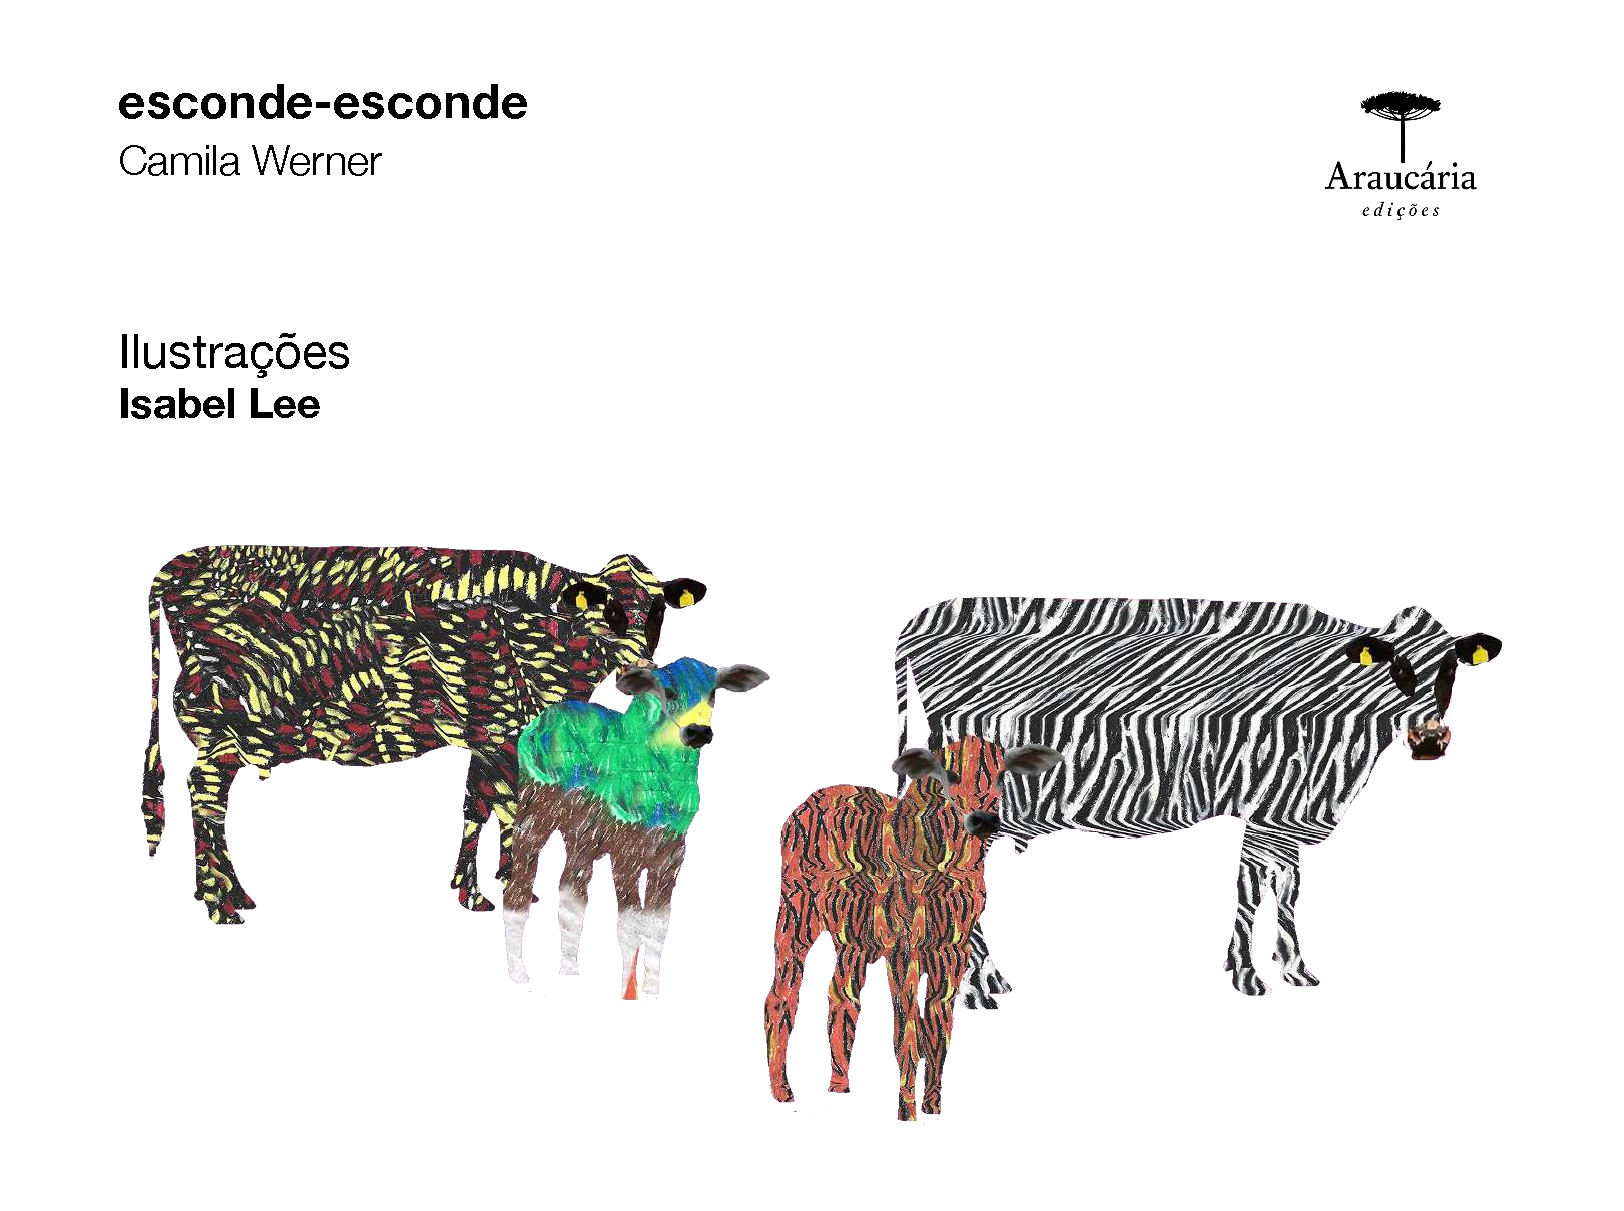
\includepdf[nup=2x2, 					% grid
			% offset=-15mm -5mm, 		% posição
			% scale=.8, 				% tamanho da página
            % delta=4mm 4mm, 			
            % frame,
            % pages={1-4}]{pdfs/PNLD2022-002_MIOLO.pdf}

\end{document}
